\chapter{Обзор} \label{chapt_review}

\TODO{TODO: Написать вводную для обзорной главы с перечислением всего обозреваемого.}


\emph{Заметки на полях: раскидать по кирпичу}

The CoNLL--SIGMORPHON 2018 \aka{Пример примечания не по делу. Высмотрел в SIGMORPHON 2020.}  Shared Task: Universal Morphological Reinflection

https://arxiv.org/pdf/1810.07125.pdf

Для 103 языков были даны леммы и морфологические характеристики, 
нужно было получить правильную словоформу -- это первая задача. 
Вторая -- дан фрагмент текста, нужно для слова указать его морфологические 
характеристики (и лемму?).

Разработано программное обеспечение wcorpus~\cite{vakbib_soft_wcorpus}.

Разработана программа ``New written Tver Karelian dialects wordform generator''~\cite{vakbib_soft_Tver_generator}.

\todo[color=green!40]{And a green note}

% Корпусная лингвистика
\section{Корпусная лингвистика} \label{sect_review_corpus_linguistics}

Корпусная лингвистика~--- это раздел компьютерной (прикладной) лингвистики, 
описывающий принципы и методы 
построения лингвистических корпусов (корпусов текстов)
и методы использования корпусных данных~\cite[с.~3]{Zakharov2005}, \cite[с.~407]{Kibrik2019}.

Научное значение корпусов заключается в том, что наличие корпуса обеспечивает воспроизводимость, 
возможность повторить эксперимент~\cite[с.~409]{Kibrik2019}. 
Трудность здесь может крыться в том, что <<живые>> корпусы, 
то есть те, над которыми продолжают работать исследователи, 
постоянно пополняются новыми текстами, увеличивается объём разметки. 
Этот рост корпуса может менять результаты эксперимента. 
Ситуацию здесь может спасти, во-первых, пресловутая <<сбалансированность>> корпуса (см. следующий раздел). 
Во-вторых, в достаточно больших корпусах, добавление новых данных будет небольшим 
относительно всего корпуса.\footnote{%
    %
    % Объём и в процентах новых слов в ВепКар 
    Приведём пример от противного, пример о добавлении новых данных в корпус ВепКар. 
    Были обработаны и преобразованы в машиночаемую форму словарные статьи 
    Сопоставительно-ономасиологического словаря диалектов карельского, вепсского, саамского языков (кратко, словарь СОСД)~\cite{SOSD2007}. 
    %одержащего 1500 понятий 
    %\TODO{TODO можно ли чуть подробнее о СОСД? Сколько типов связей и сколько связей он содержит? Сколько диалектов? Чем он грандиозен?} 
    До включения данных словаря СОСД система ВепКар содержала 35~098 лемм, 800 переводов.
    После обработки СОСД в ВепКар было включено 1425 понятий 
        (\TODO{одно понятие через значение связывает несколько десятков диалектов}), 
    20 тыс. лемм, связанных с понятиями, из них 16 тыс. новых (\TODO{то есть число лемм выросло на 46\% от 35 тыс.}); 
    130 тыс. переводов (связей между значениями лемм из разных языков, наречий). 
    При этом было создано 60 тыс. связей между значениями лемм и словами из текста, 
    50 тыс. слов в текстах получили новые связи. Но только 2 тыс. слов до этого не имели разметки вообще.
    Эти цифры говорят и о том, что Сопоставительно-ономасиологический словарь был грандиозным проектом, 
    содержащим результаты работы большого коллектива учёных, и о том,
    что корпус ВепКар ещё далёк от насыщения по числу слов и текстов.
}

 
%
% Репрезентативность и сбалансированность корпуса, достоверность данных

\subsection{Репрезентативность (и сбалансированность?) корпуса, достоверность данных} \label{sect_corpus_representativeness}

Репрезентативность 
(не путать с представительностью)\footnote{Представительный корпус -- 
это корпус, обеспечивающий максимально широкое покрытие  
различных типов текстов и функциональных стилей~\cite{Sharov2004}.
} 
корпуса (текстовых примеров) 
эмпирически определяют тем, в какой степени эти примеры показывают 
вариативность исследуемого явления~\cite{Biber1993representativeness}. 
Из этого определения следует, что нельзя говорить об универсальной 
представительности корпуса, но можно говорить 
о степени репрезентативности корпуса при решении конкретной лингвистической задачи.

В работе~\cite{Belikov2013}
оценивается достоверность корпусных исследований. 
Часто исследователи подвержены соблазну распространить опыт, полученный на конкретном корпусе, 
на весь язык, что неправомерно~\cite{Belikov2013}.

Каковы границы применимости разрабатываемого Открытого корпуса вепсского и карельского языков? 
Для ответа на этот вопрос нужно определить, тексты каких жанров и в какой пропорции включены в корпус ВепКар. 
Объём корпуса ВепКар составляет соответственно 2~677 текстов и 960~553 слов в текстах\footnote{ Данные на 23 апреля 2020~г. Cм. подробнее 
\href{http://dictorpus.krc.karelia.ru/ru/stats/by\_corp}{http://dictorpus.krc.karelia.ru/ru/stats/by\_corp}.}.

На рисунках \ref{fig:text_distr_by_corpus} и \ref{fig:text_distr_by_genre} показано распределение текстов по подкорпусам и жанрам для вепсского языка и наречий карельского языка\footnote{ Данные на 23 апреля 2020~г. Cм. подробнее 
			\href{http://dictorpus.krc.karelia.ru/ru/corpus/corpus}{http://dictorpus.krc.karelia.ru/ru/corpus/corpus}.}.

\begin{figure}
    \centering
    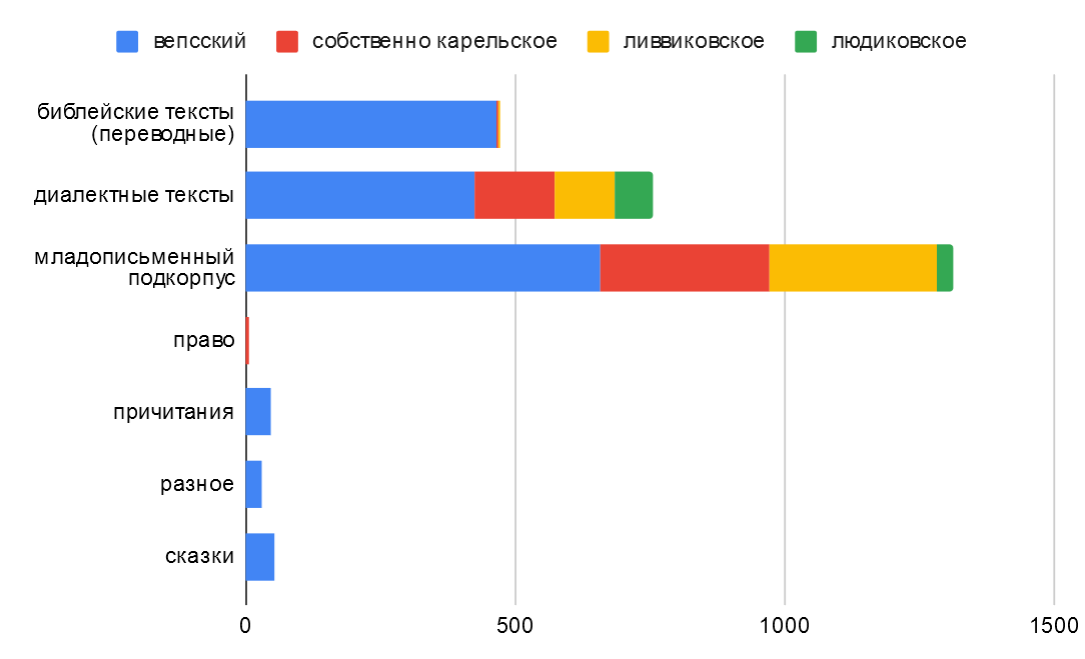
\includegraphics[width=1.0\textwidth,keepaspectratio=true]{text_distr_by_corpus.png}
    \caption{Распределение текстов по подкорпусам (вепсский язык и наречия карельского языка).}
    \label{fig:text_distr_by_corpus}
\end{figure}
%\bigskip

\begin{figure}
    \centering
    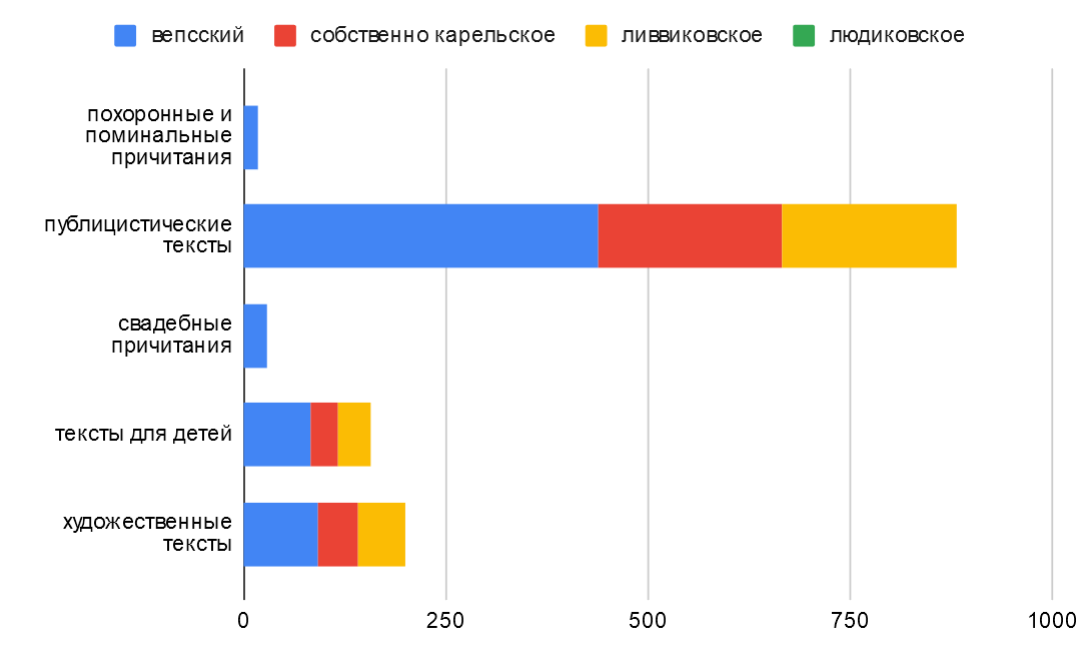
\includegraphics[width=1.0\textwidth,keepaspectratio=true]{text_distr_by_genre.png}
    \caption{Распределение текстов по жанрам (вепсский язык и наречия карельского языка).}
    \label{fig:text_distr_by_genre}
\end{figure}

Анализ временной динамики корпуса ВепКар показан на рисунке \ref{fig:text_distribution_by_date}. 2041 текстов (86,67\%) не имеют информации о дате записи.
\begin{figure}
    \centering
    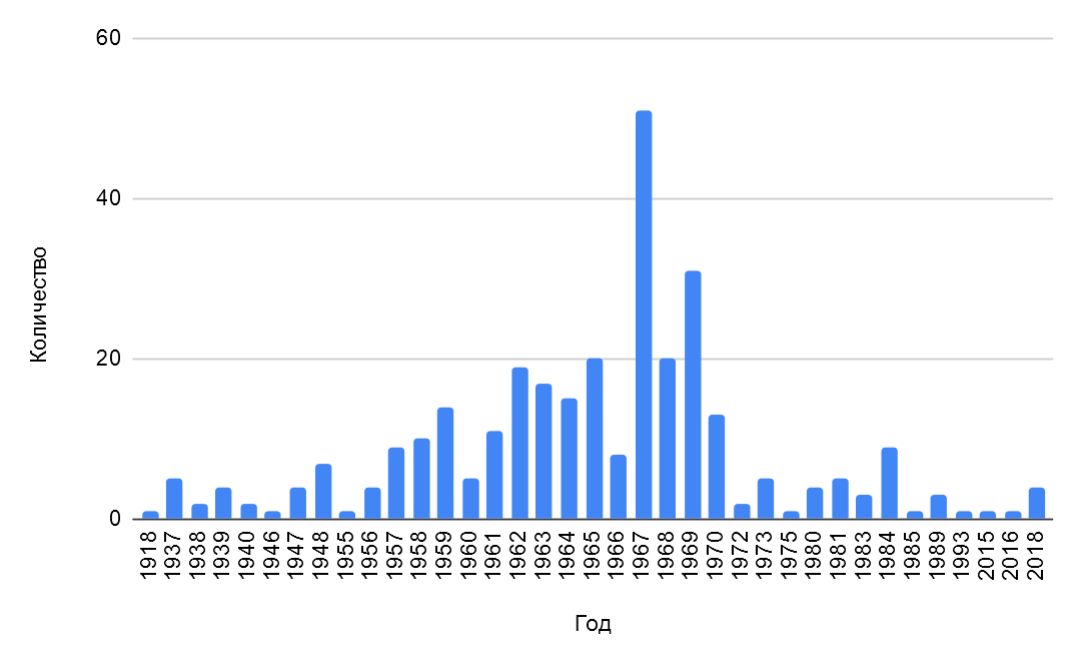
\includegraphics[width=1.0\textwidth,keepaspectratio=true]{text_distribution_by_date.png}
    \caption{Распределение числа текстов по годам.}
    \label{fig:text_distribution_by_date}
\end{figure}

Своевременно ли говорить о сбалансированности и представительности корпуса ВепКар? Вопрос остаётся открытым, нужны дополнительные исследования.
%Ответом может послужить информация о доле слов из словаря, употреблённых в текстах корпуса. 
\nata{TODO: Подсчитать долю / процент слов (для каждого из языков), которые встречаются в текстах. Процент + абсолютное число слов словаря в текстах.}
(Добавить эту статистику в корпус?)


 
%
% Примеры лингвистических корпусов
 \subsection{Примеры лингвистических корпусов}

 \subsubsection{Europarl Corpus and Words2Grids}

В работе~\cite{Fam2018tools} различают две структуры: \emph{Paradigm tables} 
и \emph{Analogical grids}. 

На языке Python разработана программа Words2Grids, которая по списку словоформ 
создаёт Analogical grids, которые, в свою очередь, нужны для создания 
таблиц склонений, то есть Paradigm tables.

Эксперименты проводились на 11 языках в корпусе текстов Europarl. 
Особняком стоят результаты по финскому (агглюнативному) языку (см. табл. 1 на с. 1063).


\subsubsection{Морфологическая разметка ГИКРЯ}

Читать и писать о работе~\cite{Selegey2016}...

\subsubsection{Корпуса уральских языков Поволжья}
Т. Архангельским разработаны веб-корпусы для пяти уральских языков\footnote{См. \url{http://volgakama.web-corpora.net}}: коми-зырянский, луговой марийский, мокшанский, удмуртский, эрзянский~\cite{Arkhangelskiy2020}. Удмуртский корпус разрабатывался в соавторстве с М. Медведевой, данные для звуковой части удмуртского корпуса собрала Е. Георгиева. Корпусы также включают тексты, извлечённые из публичных записей в соцсетях (в основном ВКонтакте), поэтому представленный язык близок к разговорной речи. Для каждого языка был разработан морфологический анализатор на основе правил. Анализаторы работают по данным словарей, поэтому в корпусах не распознаны несловарные слова или слова с опечатками. Проанализировано от 80\% до 96\% слов в корпусах. В основном контекст при морфологическом анализе не учитывается и анализатор выдаёт все возможные леммы для данной словоформы~\cite[58--59]{Arkhangelskiy2020}. Для малоресурсных языков важно, чтобы при автоматическом морфологическом анализе сохранялись в разметке все возможные формы слова для последующей проверки и выбора правильной формы лингвистом~\cite[61]{Arkhangelskiy2020}. Архангельский Т. называет такой корпусный менеджер в корпусе «дружественным к неоднозначности».

Жанровое разнообразие этих пяти корпусов таково. Основную массу составляют тексты электронных газет и журналов. Также корпусы включают художественную литературу, научные статьи, переводы Библии, статьи Википедии и официальные тексты. Большинство текстов написаны в 2010-2019 годах~\cite[59]{Arkhangelskiy2020}.

\subsubsection{Томский диалектный корпус}
Очень детальная семантическая разметка по жанрам и тематикам проведена в Томском диалектном корпусе~\cite{Zemicheva2019}.
Томский  диалектный  корпус\footnote{ См. http://losl.tsu.ru/corpus/demo}  создаётся  с  2017  г.  на  материале  диалектологических  экспедиций  в  среднеобский  регион  (Томская,  центральная  часть  Кемеровской  области).  Объём  ресурса на  апрель 2020 года более 1.7 млн словоупотреблений. Корпус имеет большой временной охват (70 лет) и детальную тематическая разметка (73  темы). 
 
%
% Компьютерная морфология
\section{Компьютерная морфология}\label{sect_review_comp_morphology}

Морфология -- это раздел лингвистики, изучающий структуру слова и его грамматические значения~\cite{MitreninaNikolaevLando2016}. Другими словами, морфология изучает
1) часть речи,
2) словоизменение,
3) словообразование,
4) грамматическое значение (что слово означает в предложении).

Компьютерная морфология анализирует и синтезирует слова программными средствами~\cite{MitreninaNikolaevLando2016}.

В компьютерной морфологии взаимосвязаны три базовых понятия: лемма, граммема и словоформа.
\begin{enumerate}
    \item \emph{Лемма}~-- это базовая, каноническая форма слова.
        Например, инфинитив у глагола.

    \item Грамматическое значение представляется в виде набора \emph{граммем}.
        Граммему также называют грамматической характеристикой,
          морфологическим признаком, морфологическим свойством,
          тегом (при разметке текста).
        Граммемы группируются по категориям (падеж, время и т.~д.).
        Одна и та же форма слова не может иметь две граммемы одной категории
        (например, глагол не может иметь сразу форму прошлого и настоящего времени).
        С другой стороны, формы могут совпадать, и их нужно уметь различать.

    \item \emph{Словоформа}~-- это\ldots \TODO{TODO}
\end{enumerate}

\emph{Лингвистическа разметка}~--- это процесс или результат 
приписывания текстам и их компонентам специальных меток, 
позволяющих выполнять поиск по лингвистическому корпуса~\cite[415]{Kibrik2019}.
%
В корпусной лингвистике есть ряд требований к разметке, известных как 
семь максим Лича~\cite[415--416]{Kibrik2019}. 


\subsubsection{Морфологическое словоизменение и морфологический анализ}

Морфологическое словоизменение\footnote{%
    \emph{Морфологическое словоизменение} по-английски звучит как
    ``inflectional morphology''.
    \emph{Система} и \emph{задача морфологического словоизменения}
    будут переводиться как
    ``morphological inflection system'' и ``morphological inflection task'' соответственно,
    см. например, американскую статью~\cite{King2020seq2seqRussianMA}.
} или просто словоизменение~--
это отображение лемм и набора морфологических признаков
на соответствующую словоформу~\cite[2821]{Cruz-Anastasopoulos-Stump2020Chatino}.

Под \emph{морфологическим анализом} слова или словоформы (morphological analysis)
подразумевается определение леммы и
грамматических характеристик словоформы~\cite{MitreninaNikolaevLando2016}.

Таким образом, если задачу <<морфологического словоизменения>> обозначить как прямую
(по лемме и признаку нужно найти словоформу),
то <<морфологический анализ>> (по словоформе требуется найти
лемму и морфологические свойства) будет обратной задачей.

\begin{figure}
    \centering
    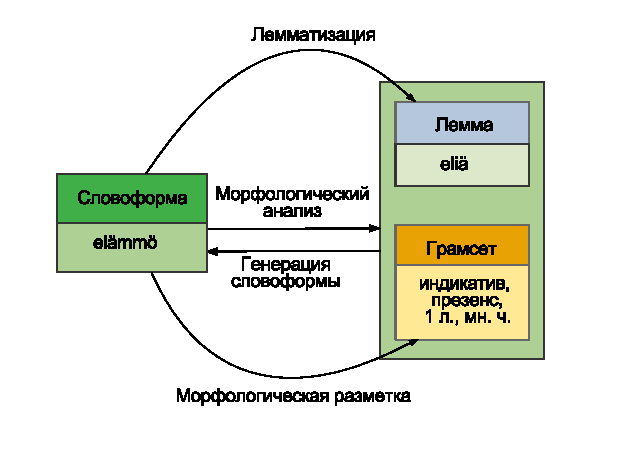
\includegraphics[width=0.75\textwidth,keepaspectratio=true]{inflectional_operations_v2}
%      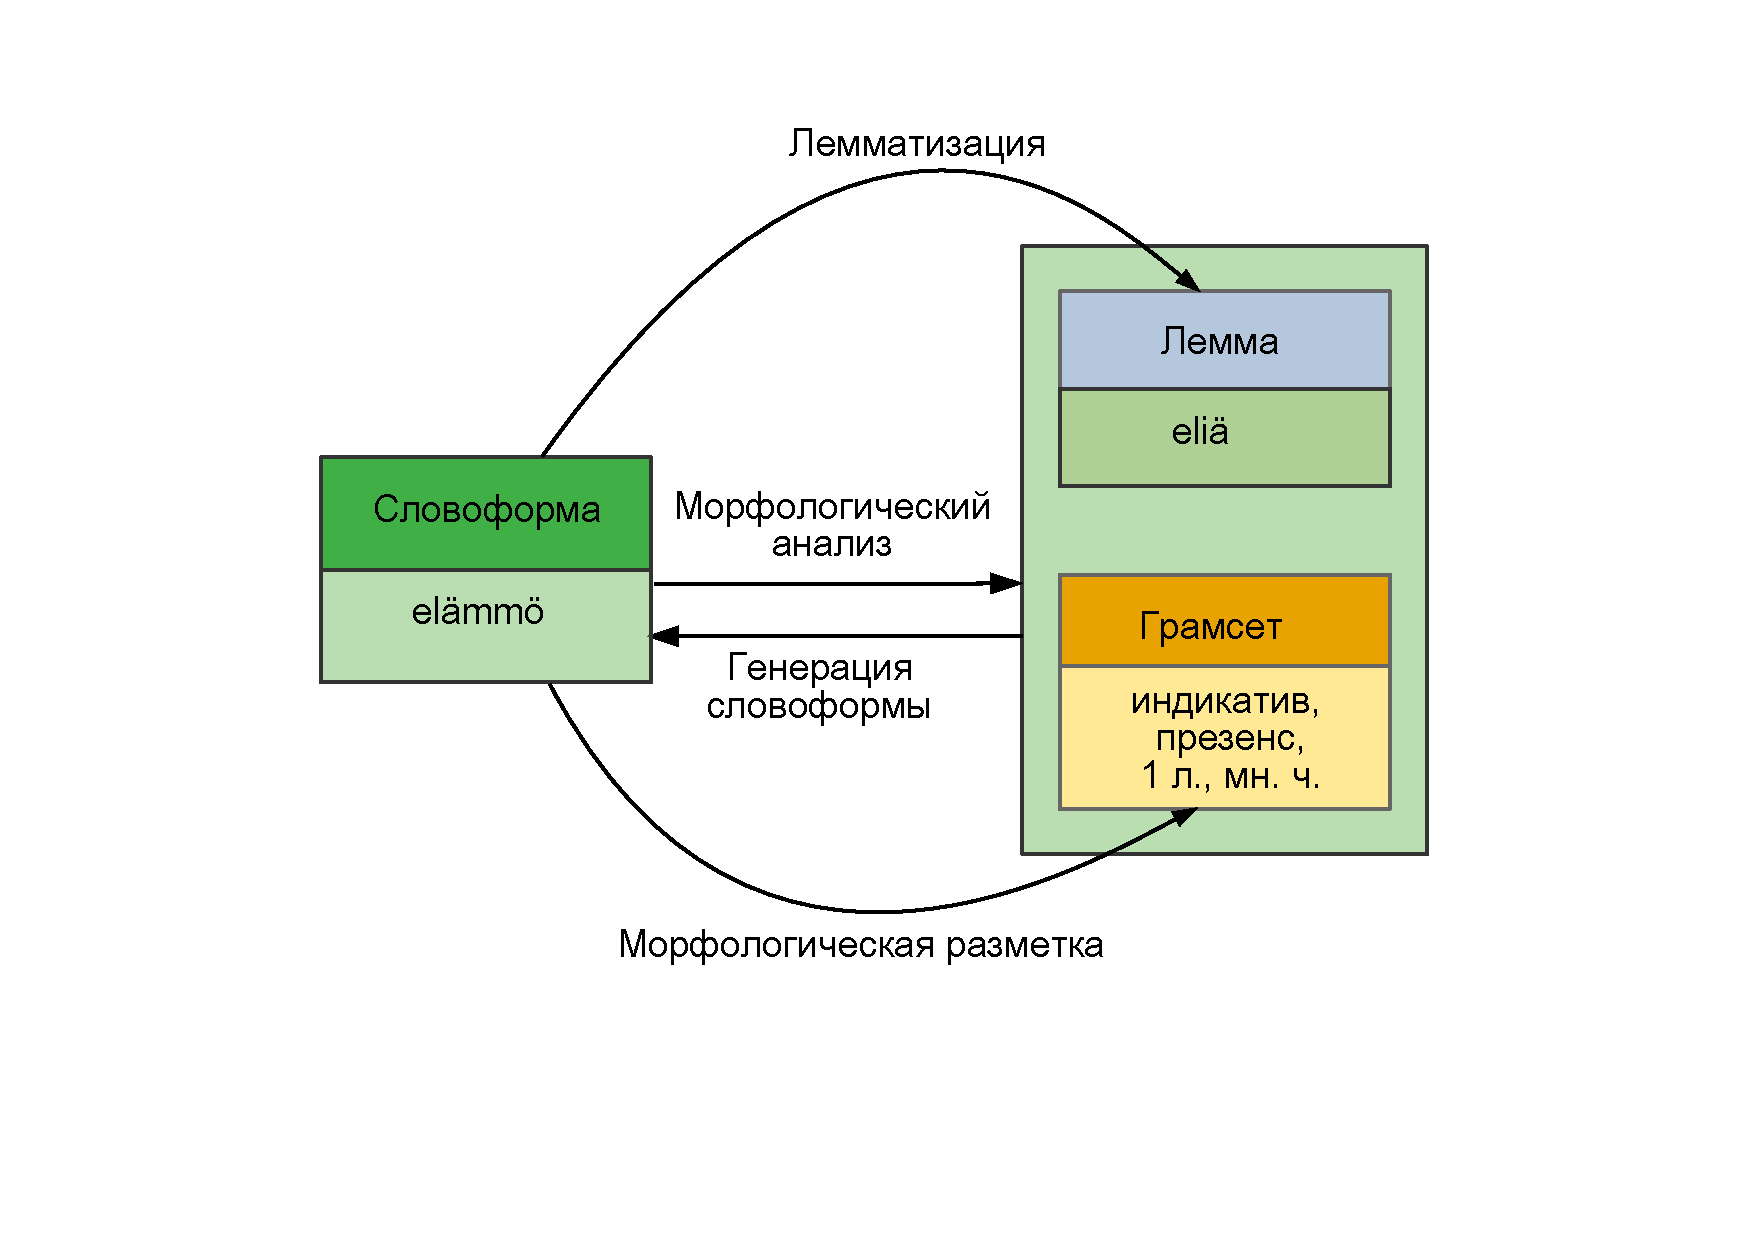
\includegraphics[width=1\linewidth]{inflectional_operations.pdf}
\caption{Четыре морфологические операции: генерация, анализ, лемматизация и разметка 
		   на примере карельского глагола ``eliä'' (жить).  
              Адаптация рисунка из статьи~\cite{Nicolai2020FineGraned}.} \label{fig:inflectional_operations}
\end{figure}

Отметим, что в ряде языков отсутствует морфологическое словоизменение,
например, в языках йоруба и севернокитайском~\cite[2]{Vylomova2020Sigmorphon}.




\subsubsection{Paradigm Cell Filling Problem}

С задачей морфологического анализа тесно связана задача
``a paradigm cell filling problem'' (PCFP)~\cite{Ackerman08PartsAndWholes}.



\subsubsection{Соревнования по морфологическому анализу (и результаты?)}

Рассмотренные выше задачи решают на соревнованиях
между компьютерными программами в рамках различных конференций:
\begin{description}[align=left]
    \item [Диалог]\footnote{См. \url{http://www.dialog-21.ru}}~--
            известная отечественная конференция
            по компьютерной лингвистике.
            В 2019 году в преддверии этой конференции
            было проведено соревнование LowResourceEval
            по анализу нескольких языков России~\cite{Klyachko2019LowresourceEval}.
        \TODO{TODO коротенько о главных результатах.}

    \item [SIGMORPHON]\label{SIGMORPHON}\footnote{См. \url{https://sigmorphon.github.io}}~--
                это группа учёных (одна из множества групп ACL\footnote{%
                ACL расшифровывается как ``Association for Computational Linguistics''.
                Ассоциация компьютерной лингвистики~-- это
                международное научное и техническое сообщество специалистов
                по обработке текстов и языковой информации.
            }),
            занимающихся вычислительной морфологией и фонологией,
            и одноимённая конференция, проводимая этими учёными.
            В соревновании по морфологии ``SIGMORPHON 2020''
            были использованы данные
            разрабатываемого корпуса ВепКар~\cite{Vylomova2020SIGMORPHON}.

            \TODO{TODO коротенько о главных результатах.}
\end{description}



\subsection{Малоресурсные языки}\label{sect_low-resource}

Языки, которым посвящена эта работа, то есть вепсский и карельский,
относят к малоресурсным языкам~\TODO{TODO: доказательная ссылка}.

Есть интуитивное представление, что \emph{малоресурсные языки}~---
это языки, обладающие недостаточным объёмом текстов
в бумажном и электронном виде,
имеющие слабую компьютерную поддержку.
То есть для таких языков может не быть
электронных словарей, лингвистических корпусов,
систем проверки правописания, систем машинного перевода,
либо они есть, но несопоставимы по качеству и объёму с теми же объектами
высокоресурсных языков.
\TODO{TODO: сделать таблицу с рядом языков России
и наличием таких ресурсов у них. И решением
о мало-, высокоресурсности языков.}.

В работе~\cite{Anastasopoulos2019Pushing_Limits_Low-Resource_MI}
предложены численные границы для этих двух видов языков.
Малоресурсные языки содержат около 100 примеров в обучающем наборе
и 50-100 (редко 1000) примеров в настраивающем наборе данных\footnote{%
    В машинном обучении обычно выделяют три типа
    последовательно используемых данных: training, validation и test sets.
    \begin{enumerate}[label=(\roman*)]
        \item \emph{training set} (тестовый набор данных)~--
            это набор данных для настройки весов, например, матрицы,
            где эти веса вычисляются с помощью нейронных сетей.

        \item \emph{validation set, development set, dev set}
            (настраивающий или настроечный набор данных)~--
            набор данных для настройки гиперпараметров нейронной сети,
            например, число нейронов в каждом слое.

        \item \emph{test set} (тестовый набор данных)~-- это набор данных
            для оценки полученной модели.
    \end{enumerate}
    }% eo footnote
%
.
Большинство высокоресурсных языков содержат по 10\,000 примеров.
Эти цифры приводятся на примере данных,
предоставленных участникам соревнования SIGMORPHON 2019 года\footnote{%
    См. о SIGMORPHON на с.~\pageref{SIGMORPHON}.
    Данные соревнования ``SIGMORPHON 2020 task 0'', представленные
    в таблице \TODO{(TODO ссылка на таблицу)},
    доступны по
    ссылке~\url{https://github.com/sigmorphon2020/task0-data}.
}~\cite{Anastasopoulos2019Pushing_Limits_Low-Resource_MI}.


\TODO{Перевести данные в табличку с размерами train, dev и test set для языков 
ВепКар на SIGMORPHON 2020
И на основе этого сделать вывод, какие из наших языков мало- или много- 
ресурсные.}

SIGMORPHON 2020 task 0

vep  train 94\,395 dev 13\,320 test 26\,422

krl  train 80\,216 dev 11\,225 test 22\,290

olo  train 43\,936 dev 6\,260 test 12\,515

lud  train 294 dev 41 test 82

\begin{table}
%\begin{adjustbox}{width=1\textwidth}
\small
\centering
\small
\begin{tabular}{c|r|r|r|r|r|r|>{\hspace{2em}}r|r|>{\hspace{2em}}r|r}
\toprule
%\multicolumn{1}{c}{\textbf{Lang}}&\multicolumn{3}{c}{\textbf{Total}}\\
\textbf{Язык / Наречие} & \textbf{Код языка} & \textbf{Train} & \textbf{Dev} & \textbf{Test} \\
%\cmidrule(lr){1-1} \cmidrule(lr){2-4} \cmidrule(lr){5-7} \cmidrule(lr){8-9} \cmidrule(lr){10-11}
% &Train& Dev & Test \\

\midrule
Карельский & krl&80216&11225&22290\\
 lud&294&41&82\\
 olo&43936&6260&12515\\
 vep&94395&13320&26422\\
%\midrule
%est&26728&3820&7637&2.7&0.4&0.8&6.1&5.1&22.4&11.6\\
%fin&99403&14201&28401&0.0&0.0&0.0&0.0&0.0&32.6&17.2\\
%izh&763&112&224&0.0&0.0&0.0&0.0&0.0&42.9&22.3\\
%liv&2787&398&802&0.0&0.0&0.0&0.0&0.0&40.7&24.1\\
%\midrule
%ang&29270&4122&8197&11.8&1.8&3.4&21.6&21.9&35.1&21.3\\
%aze&5602&801&1601&11.9&1.9&4.0&22.3&20.9&31.5&20.2\\
%cre&4571&584&1174&18.5&2.1&4.9&29.8&29.6&5.5&2.7\\
%dan&17852&2550&5101&16.5&2.5&5.0&34.5&32.9&71.4&51.8\\
%nob&13263&1929&3830&10.5&1.8&3.1&18.5&19.7&80.5&70.5\\
%pei&10017&1349&2636&15.8&2.6&4.9&21.5&21.4&9.1&4.7\\
\bottomrule
\end{tabular}
%\end{adjustbox}
\caption{Number of samples in training, development, test sets, as well as statistics on systematic errors (inconsistency) and percentage of samples with lemmata observed in the training set.
(VepKar languages, other Uralic languaes and languages with the highest rates of inconsistency, todo ref to SIGMORPHON2020)
}
\label{tab:lang-stats}
\end{table}

\newpage\clearpage


\begin{tabular}{llr}
\hline
\multicolumn{2}{c}{Item} \\
\cline{1-2}
Animal    & Description & Price (\$) \\
\hline
Gnat      & per gram    & 13.65      \\
          & each        & 0.01       \\
Gnu       & stuffed     & 92.50      \\
Emu       & stuffed     & 33.33      \\
Armadillo & frozen      & 8.99       \\
\hline
\end{tabular}






\subsection{Вепсский и карельский языки}\label{sect_review_veps_karelian}


\subsubsection{Чудное введение в базовые терминология: лемма, лексема и тратата}

\TODO{TODO: см. http://macrocosm.narod.ru/lingvo.html}


\subsubsection{Богатые тоже плачут (богатая морфология), мексиканское чатино и все-все-все}

Вепсский и карельский языки являются языками с богатой морфологией.
\TODO{TODO: привести число словоформ в парадигме именной и глагольной формы языков. В виде таблицы? Ссылка на нашу статью?}

Моделирование грамматических функций (modeling of the grammatical functions)
для языков с богатой морфологией (rich morphology
\TODO{TODO: Дать определение <<богатой морфологии>>}
) крайне важно.
Это особенно трудная и важная задача
для малоресурсных языков~\cite[2820]{Cruz-Anastasopoulos-Stump2020Chatino}.


%Let us describe several works devoted to the development of morphological analyzers for the Veps and Karelian languages.
Опишем несколько работ, посвящённых разработке морфологических анализаторов вепсского и карельского языков.
\begin{itemize}
%  \item The Giellatekno language research group is mainly engaged in low-resource languages, the project covers about 50 languages~\cite{Moshagen2014}. Our project has something in common with the work of Giellatekno in that (1) we work with low-resource languages, (2) we develop software and data with open licenses.
  \item Основным предметом исследования языковой группы Giellatekno 
      являются малоресурсные языки.  
        Разработаны лингвистические ресурсы 
        для порядка 50 языков~\cite{Moshagen2014}. 
        Общее в нашей работе с исследователям из Giellatekno в том, что 
        (1) мы также работаем с малоресурсными языками, 
        (2) мы разрабатываем программное обеспечение 
        и публикуем словари и корпуса текстов с открытой лицензией.
      Ключевую роль в разрабатываемых в Giellatekno языковых технологиях 
        играют формальные подходы. 
        В Giellatekno работают с морфологически богатыми языками.
        Для анализа и генерации словоформ (морфологический синтез и анализ) 
        они используют конечные преобразователи 
        (FST или finite-state transducers)~\cite{Moshagen2014}. 
% 
%  \item There is a texts and words processing library for the Uralic languages called UralicNLP~\cite{UralicNLP2019Hamalainen}.
%  This Python library provides interface to such Giellatekno tools as FST for processing morphology and constraint grammar for syntax. 
%  The UralicNLP library lemmatizes words in 30 Finno-Ugric languages and dialects including the Livvi dialect of the Karelian language (\textit{olo} -- language code).
  \item Для обработки слов и текстов на уральских языках разработана 
      библиотека UralicNLP~\cite{UralicNLP2019Hamalainen}. 
        Эта библиотека на языка Python предоставляет интерфейс 
        к конечным преобразователям Giellatekno 
        и к грамматикам ограничений (constraint grammar) той же системы. 
        Программный код библиотеки доступен 
        онлайн\footnote{См. \url{https://github.com/mikahama/uralicNLP}}.
        Библиотека UralicNLP выполняет лемматизацию слов 
        для 30 финно-угорских языков, включая 
        ливвиковское наречие карельского языка (языковой код \textit{olo}).
\end{itemize}





\bigskip
По точности результаты по языку Чатино значительно хуже
средних результатов соревнования ``SIGMORPHON 2019'' по 66 языкам.
Это косвенно указывает на сложность морфологии языка~\cite[2822]{Cruz-Anastasopoulos-Stump2020Chatino}.
\TODO{TODO: Данные о чатинском языке приведены по статье 2019 года McCarthy.
            Для вепсского взять те же данные из статьи~\cite{Vylomova2020SIGMORPHON}.}


\subsubsection{Открытые ресурсы по карельскому и вепсскому языку в интернете} \label{sect_open_krl_vep_inet}

В статье сотрудников Google~\cite{Prasad2018} перечислены открытые ресурсы для языков мира.
Посмотреть эти ресурсы и перечислить - где и сколько есть текстов и статей
для карельского и вепсского языков. Сравнить (в процентах) с тем, что есть
в электронном виде в ВепКаре, в бумажном виде в ИЯЛИ.

%@article{prasad2018mining,
%  title={Mining Training Data for Language Modeling Across the World's Languages},
%  author={Prasad, Manasa and Breiner, Theresa and van Esch, Daan},
%  year={2018}
%}







\subsection{Обзор компьютерных программ для морфологической обработки}

\subsection{Финский язык}\label{sect_review_fin}

Статья о лемматизаторе FinnPos~\cite{silfverberg2016finnpos}.

%https://github.com/mpsilfve/FinnPos

%
% Конечный преобразователь (трансдьюсер) и конечные автоматы
\section{Конечные преобразователи и автоматы} \label{sect_review_automaton}

Математические основы конечных автоматов и трансдьюсеров были разработаны 
несколько десятилетий назад~\cite{MohriChapter4Lothaire2005applied}.
%Lothaire2005applied}.


Вилфред Брауэр. Введение в теорию конечных автоматов. М.: Радио и Связь 392 с; 
1987 г. \todo{Прочитать (см. отечеств. терминологию, в библиотеке или libex).}

%Разработано программное обеспечение wcorpus~\cite{vakbib_soft_wcorpus}.


\subsection{Взвешенные трансдьюсеры} \label{sect_weighted_transducers}

Трансдьюсеры могут использоваться для отображения и связывания разных видов данных, 
например, слова и последовательности фонем. 
Подобные автоматы нужны при разработке систем распознавания речи~\cite[с.~200]{MohriChapter4Lothaire2005applied}.

Веса позволяют указать в такой модели отображения наличие неопределённости. 
Например, во взвешенных трансдьюсерах одному слову могут отвечать несколько вариантов 
произношения слова с разными рангами или вероятностями~\cite[с.~200]{MohriChapter4Lothaire2005applied}.


Базовые положения о морфологических трансдьюсерах в статье "Carlson, L., 2005. Inducing a morphological transducer from inflectional paradigms. Inquiries into Words, Constraints and Contexts, p.18-24."
%см. /data/all/docs/science/linguistics/finite-State-Transducers/about/morpho_from_paradigm_2005_Lauri_Carlson_42-48.pdf


История вопроса о конечных преобразователях с 1980 по 2005 год.
\todo{Karttunen, L. and Beesley, K.R., 2005. Twenty-five years of finite-state morphology. Inquiries Into Words, a Festschrift for Kimmo Koskenniemi on his 60th Birthday, pp.71-83.}
% 25years_FSMorphology_KarttunenBeesley2005.pdf

И в целом история вычислительной лингвистики \todo{Karttunen, L., 2007. Word play. Computational Linguistics, 33(4), pp.443-467.}
% Word_play_2007Karttunen.pdf

% As many observers have indicated, the most promising approaches will probably integrate rule-based and corpus-based methods. 
Как отмечают многие наблюдатели, наиболее многообещающие подходы, вероятно, будут включать методы, основанные на правилах и корпусе~\cite{Hutchins1999}.



%\section{Software automaton} \label{sect_automaton_soft}

%В статье сотрудников Google~\cite{Prasad2018}  перечислены открытые ресурсы для языков мира. 

%и \emph{Analogical grids}. 




%
% Нейронные сети
\section{Нейронные сети} \label{sect_nn}

\subsection{Введение} \label{sect_nn_review}

Глубинные нейронные сети -- это рычаг, который, опираясь на большие массивы данных, сдвинул многие камешки-задачи в лингвистике~\cite[2827]{Cruz-Anastasopoulos-Stump2020Chatino}.

Посимвольное представление вместо пословного 
даёт преимущество при обучении нейронных сетей 
различению морфологических свойств, 
особенно при анализе редких и новых слов~\cite[868]{Belinkov2017NeuralLearnMorphology}.

При решении самых разных лингвистических задач, 
в том числе при определении части речи слова (POS tagging), 
используют \emph{векторное представление слов}\footnote{%
    Word embeddings (векторное представление слов или языковая модель)~--- 
    это представление слов в виде массива чисел (n-мерного вектора), 
    построенного с помощью 
    дистрибутивно-семантической модели 
    (distributional semantic model или DSM)~\cite[1]{SurveyDSM2018Bakarov}.
} 
и нейронные сети.


Как оценить качество построенного векторного представления? 
То есть качество построенной дистрибутивно-семантической модели. 
Этот вопрос является открытым. Методы оценки делят на~\cite{SurveyDSM2018Bakarov}:

 \emph{внешние методы оценки} (extrinsic evaluation).
 Здесь оценка внешняя относительно языковой модели. 
 Оценивается результат решения задачи, в которой используется модель. 
 Например, в POS tagging оценивается точность указания части речи.


 \emph{внутренние методы оценки}~--- \TODO{TODO: дочитать и дописать}

 

% Вывод
\section{Выводы по главе \ref{chapt_review}} \label{sect_conclusion_review}

 




